\chapter{Discussion}

The EWC paper is currently one of the most known approaches for overcoming catastrophic forgetting.
Their paper shows that it performs good on a permuted mnist dataset with three sequential learning tasks.

Sadly the paper just delivers main facts and ideas behind the EWC solution.
It leaves some important facts for understading their approaches and test benchmarks.
They do show the main idea, formula and advanatges by using them.
But they do not explain why they are using the FIM, in fact just the diagonal of the FIM.
Moreover, they leave out helpful formulas.
Their FIM is not documented and they leave out deeper calculation insights for their idea.
Even an code base is not available.
In the appendix are some parameters of their benchmarks documented.
But their benachmarks for superviseed learning (Figure \ref{fig:ewc_permuted_example}) on the mnist dataset are not reproducible.
They do not present a solution for a reasonable lambda value, learning rate or iterations for the second task.
Therefore, this article had to come up with its own benachmarks.
The benchmarks refer to the report \cite{cf_application_oriented_study} which include an application-oriented study on the EWC algorithm.
The network was given three hidden layers with 800 neurons.
This feature base is a proven structure for the mnist problem.
The iterations and batch sizes are chosen from the study \ref{cf_application_oriented_study}.
This article increased the iterations for the permuted benchmark to analyze the surpassing of the $T_2$ accuracy to the complete dataset.
lambda was default set to $\lambda = \frac{1}{learningrate T_2}$.

Currently there are multiple implementations of EWC available.
Most of them are created with PyTorch, a similar open-source machine learning library.
But there are two solutions implemented in Tensorflow and available on Github
\footnote[1]{\url{https://github.com/ariseff/overcoming-catastrophic}}
\footnote[2]{\url{https://github.com/stokesj/EWC}}.
Both show a solution for an permuted mnist on supervised learning but not a disjoint mnist.
The more popular implementation\footnotemark[1] modifies the original algorithm.
For the FIM calulation it does not use the given labels from the dataset.
It generates new labels based on a randomization of the softmax progabilities.
% Moreover, the CrossEntropy loss funtion is not properly used for calculating the gradients.
% They avoid to negate the log from CE
The second implementation \footnotemark[2] is used in the report \cite{cf_application_oriented_study}.
As discovered in Section \ref{project_review_improvements} it built a workaround to be able to perform per-gradient calculations in Tensorflow.
This code base was the inspiration for the default lambda value.
\newline
The reimplementation of EWC in Python and Tensorflow omits these drawbacks and enables the algorithm for the modification \ref{project_review_improvements}.

The baseline showed that the EWC algorithm works with the three benchmarks.
This EWC algorithm (Figures \ref{fig:ewc_d9-1}, \ref{fig:ewc_d5-5}, \ref{fig:ewc_p10-10}) shows that it reduces catastrophic forgetting (Figure \ref{fig:catastrophic_forgetting_example}).
But it does not solve catastrophic forgetting for these benachmarks on the mnist dataset.
The application-oriented study \cite{cf_application_oriented_study} discovered that EWC is in some way effective against CF for simple SLTs (D9-1 benchmark), but ineffective against CF for more complex problems (D5-5 benchmark) \cite{cf_application_oriented_study}.
The case of D5-5 they can not register any sign of learning.
After the first task, the complete dataset had an accuracy of 50\% and after the second task 31\% 
\cite{cf_application_oriented_study}.
In comparison to these results, the benchmarks in this article (Figure \ref{fig:ewc_d5-5}) show that there is a learning happending.
After the first task has the complete dataset an accurcacy of 50\% and after the second task 79\%.
\newline
The comparison of $T_2$ in Figure \ref{fig:ewc_d5-5} and $T_1$ in Figure \ref{fig:ewc_p10-10} shows that in the D5-5 benchmark it would be much easier to just train a new model with the complete mnist dataset.
Because of the same iterations, batch size and a smaller learning rate of $T_1$ (in Figure \ref{fig:ewc_p10-10}) the perfromance of training the complete dataset instead of retraining with the EWC algorithm would increase the accuracy by 15.37\%.
But these benchmarks are just a small representation of problem in large datasets and models.
In this case mnist just provides a simplification of the problem to be able to test an algorithm.
And it gives the ability to test several different parameters in a short amount of time and computation power.
So these benchmarks help to get a better understanding of the algorithm.
If the EWC would be used in real-worls scenarios, it would be used in cases, where the multitask learning (Figure \ref{fig:intro_motivation_multitask_learning_paradigm}) is not an option.

For the implementation of the EWC algorithm with Python and Tensorflow exist multiple ways.
The attached codebase \footnote{\url{https://github.com/florianwiech/incremental-machine-learning}} tried multiple implementations.
First implementations dealt with own coded dataset, iterator and network classes.
The advantage is that the developer has full control over the complete code.
A big disadvantage is though, that other developers need a lot of effort to understand the code.
This is why a developer shoul stick to given helper classes of the included frameworks.
Most of the time they present a good documentation and other developers who know the framework are able to understand the code quiet quickly.
Because of that reason the code was converted to built-in Tensorflow classes like the Dataset, Iterator and autoloading of the MNIST dataset.
This code sticks as close as possible to the Tensorflow provided classes.
But along the way of converting the code to the Tensorflow classes, the developer of the code just lost a lot of control and the ability to see what exactly being calculated by just looking at the code.
This is a huge disadvantage with the built-in classes of Tensorflow.
\newline
Through the own implementation, the option between a FIM calculation and the modification is straightforward by adjusting the "batch\_fisher" variable.
Since both computations with a batch size of 1 are the same, the modification is applied when the fisher batch size is higher than 1.

% modification
The comparison between the baseline benchmarks and experiments with the modification are looking encouraging.
…
% the comparison of fig:ewcd9-1 and exp_d9-1_bs1k results that there is nearly no difference between the FIM calc and the calculation of per batch gradients.

% plots: comparison the gradients with different batch sizes


% closer look to the differences, in fact the gradients

\iffalse
The modification of the FIM was tested in the experiments.
Let's now take a closer look to the changes between the baseline and the modifications.

The difference between these two approaches are the calculated gradients of $T_1$.
The FIM squares every gradient and the modification squares the average gradient from an batch.
So Figure \ref{fig:dis_d91,fig:dis_d55,fig:dis_d1010} show the differences of the minima and maxima by calculating the matrix with the FIM or the modification.



- compare baseline to experiments

- have a closer look to the gradients

- we see that the results are extremly similar
- pros for the modificatoin are that the computation time is a lot lower, because not so many operations

\fi

\begin{figure}[H]
    \centering
    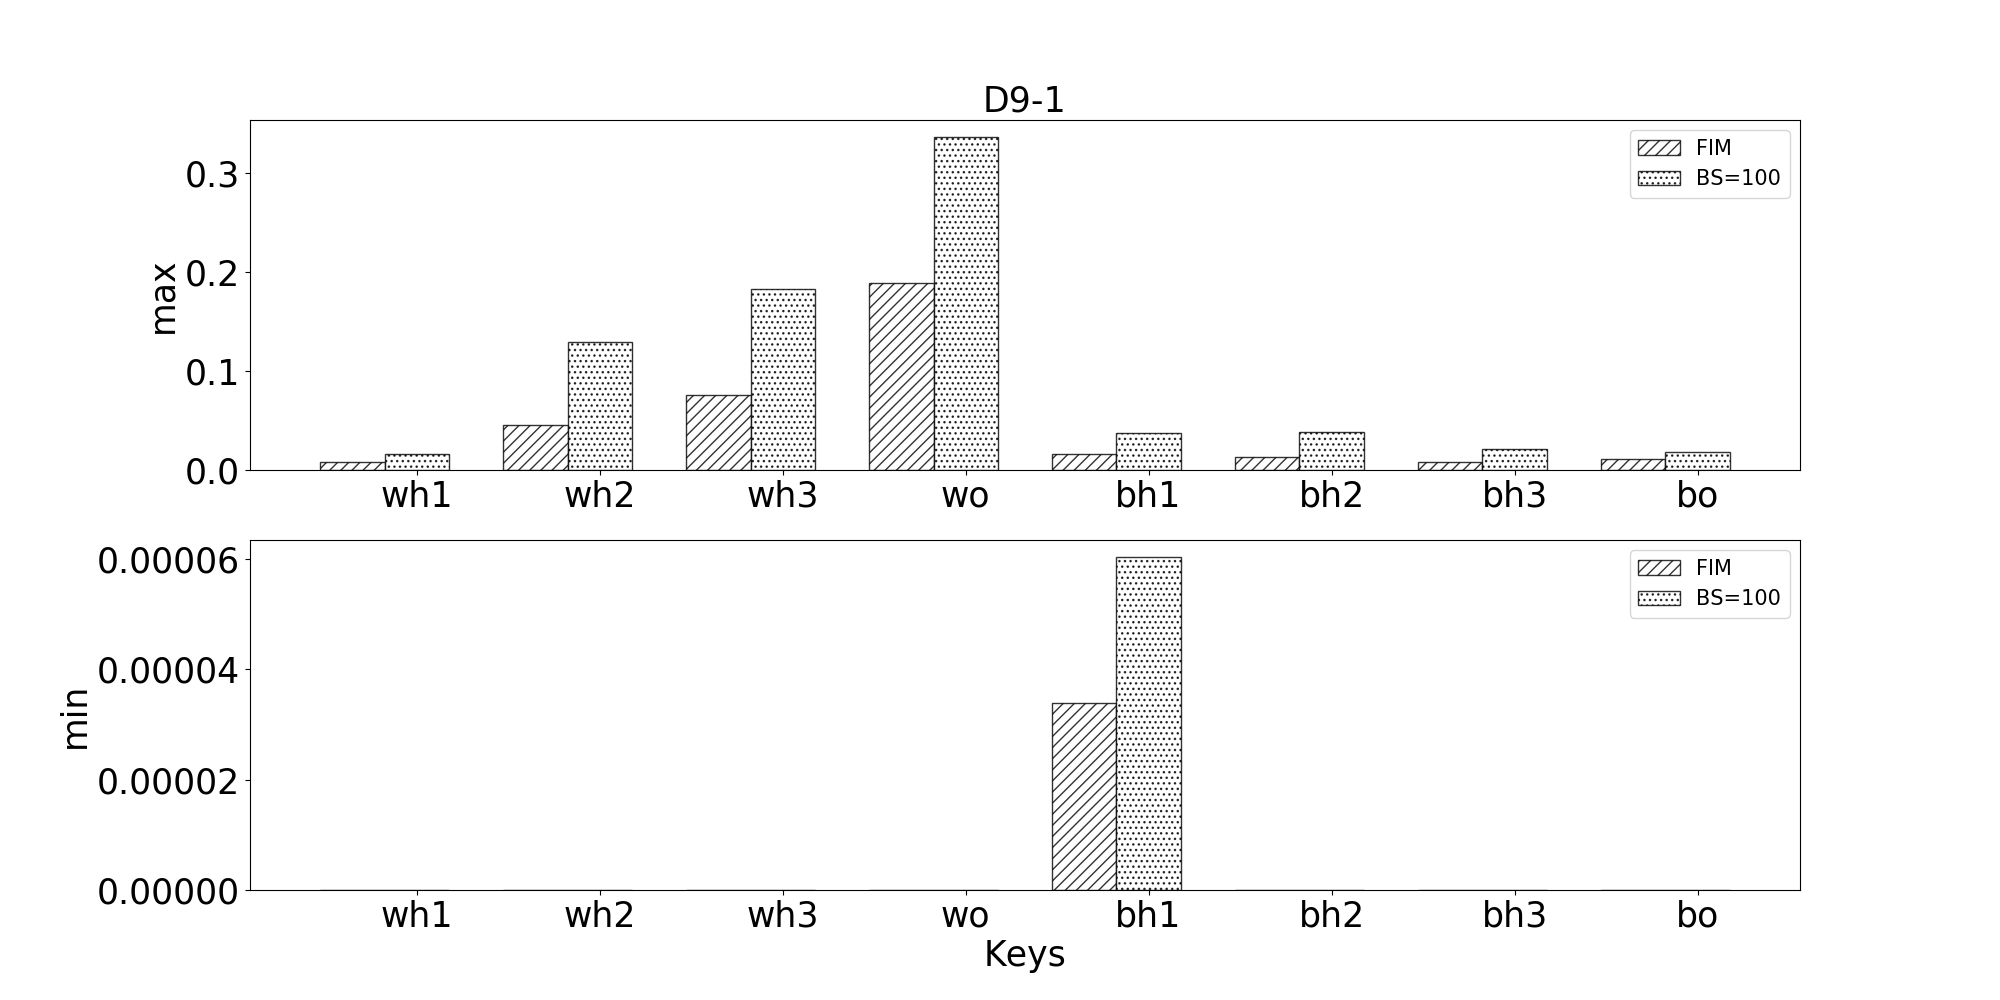
\includegraphics[width=\textwidth]{project/discussion/D91}
    \caption{D9-1 Gradients}
    \label{fig:dis_d91}
\end{figure}

\begin{figure}[H]
    \centering
    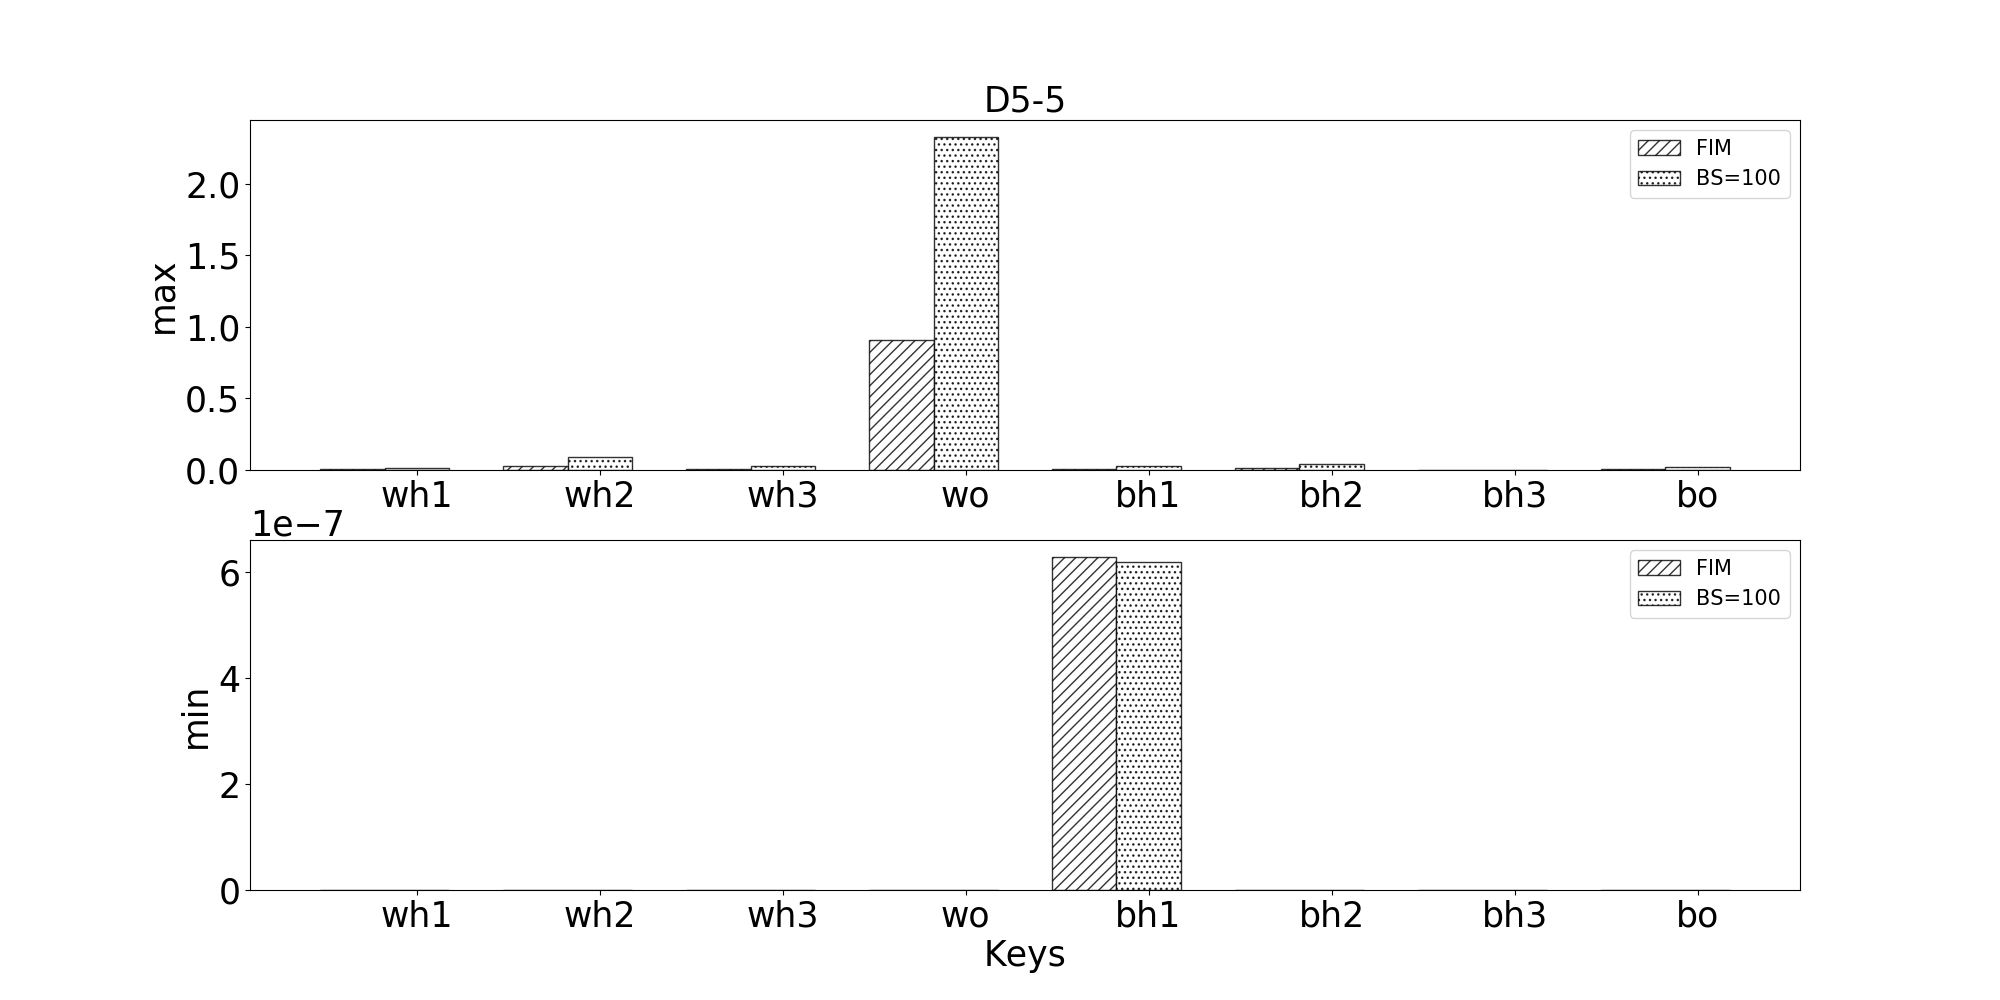
\includegraphics[width=\textwidth]{project/discussion/D55}
    \caption{D5-5 Gradients}
    \label{fig:dis_d55}
\end{figure}

\begin{figure}[H]
    \centering
    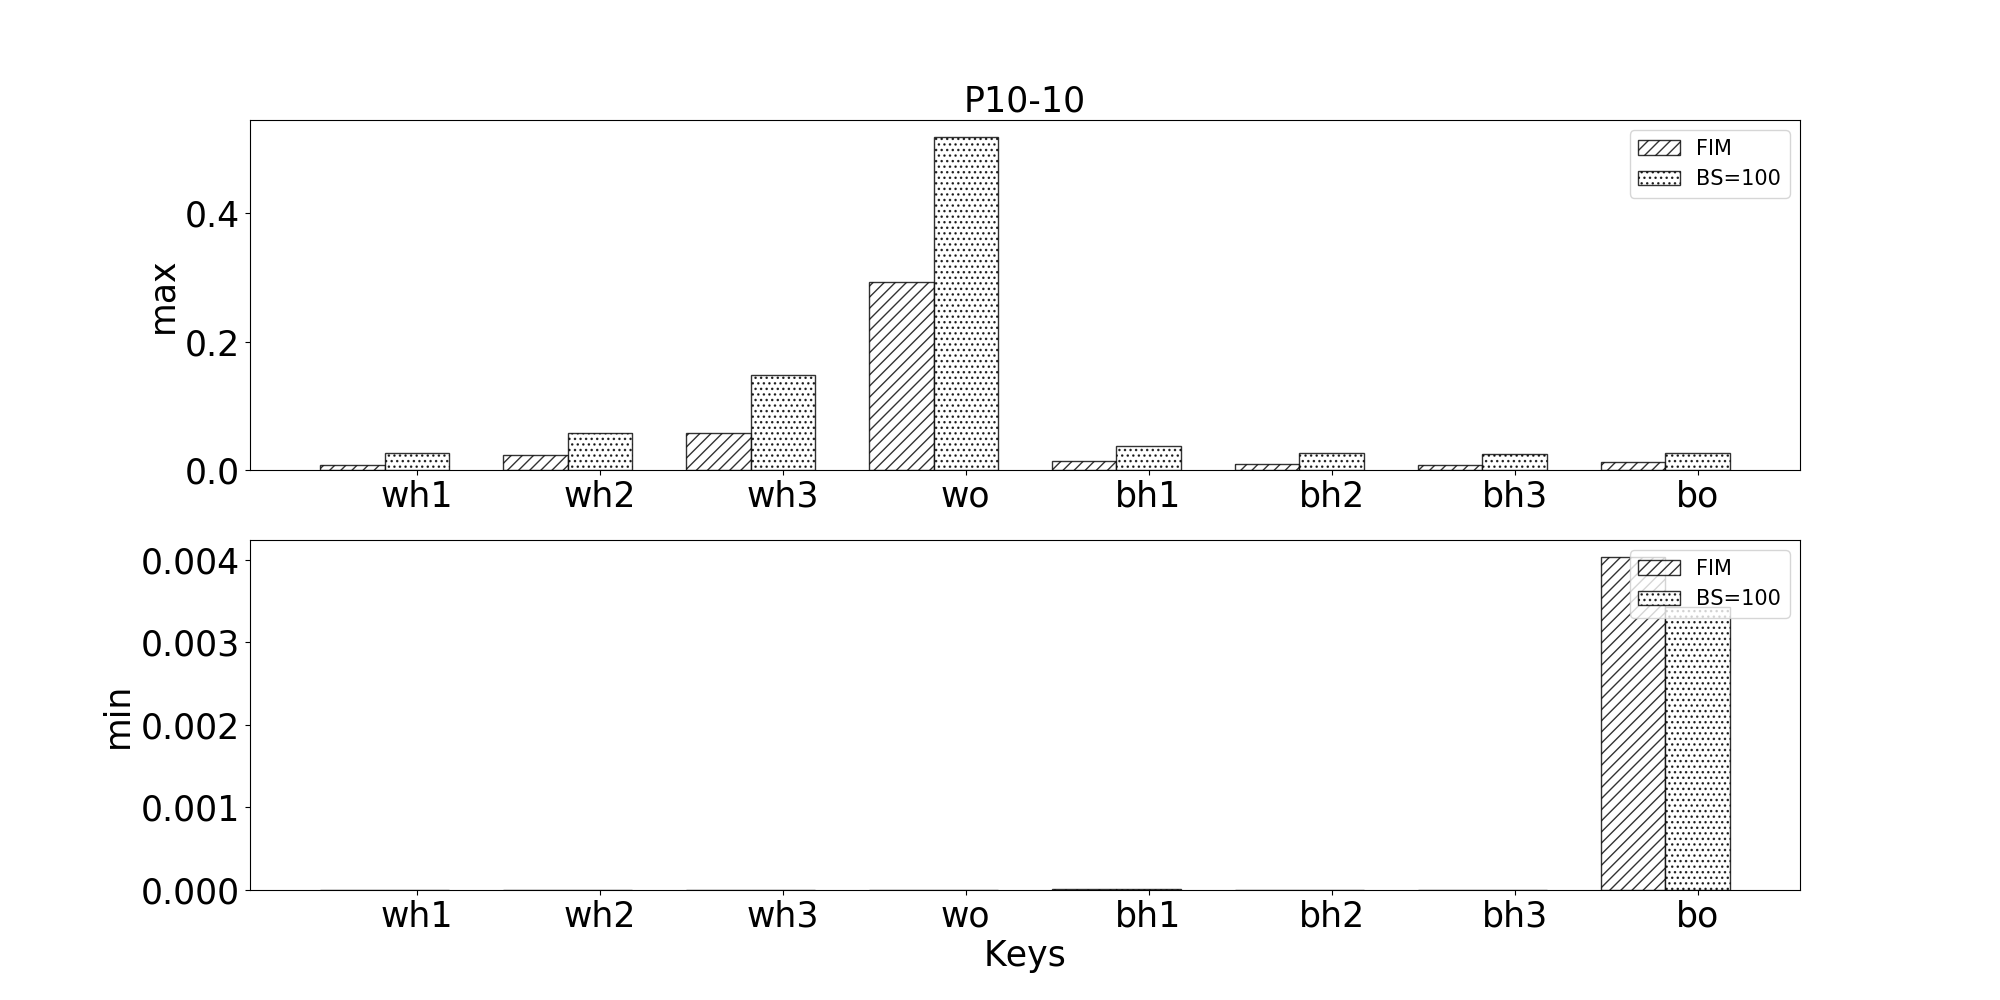
\includegraphics[width=\textwidth]{project/discussion/P1010}
    \caption{P10-10 Gradients}
    \label{fig:dis_d1010}
\end{figure}


\section{Conclusion}

% the experiments \& figueres from discussion show that the modification is possible and delivers similar results compared to the ewc from baseline.

\section{Outlook}

% test with multiple tasks and check, when the forgetting for the first task increases drastically
% just tested with fixed 2500 iterations, it should be tested with more and less iterations
% different batch sizes, because it is not per gradient anymore
% test with the modification on other datasets
% test modification on others that use fiher, like IMM or NGD
% take a closer look to lambda
%   would be useful to have a fixed lambda term
%   useless if lambda needs to be calculated for every new task…
